\documentclass[12pt,a4paper]{article}
\usepackage[UTF8]{ctex}
\usepackage{amsmath,amssymb}
\usepackage{xcolor}
\usepackage{hyperref}
\usepackage{geometry}
\usepackage{graphicx}
\geometry{margin=2.5cm}

\title{Quantum Curve Fitting / 量子曲线拟合}
\author{QuoNic}
\date{}

\begin{document}
\maketitle

\begin{center}
\textbf{ML / 机器学习} | 难度：高级 | 预计时间：20 分钟
\end{center}

\tableofcontents
\newpage

\section{为什么需要？}

量子曲线拟合是经典曲线拟合的量子推广，用于在量子环境中拟合数据。

\subsection{经典局限}
\begin{itemize}
  \item 经典曲线拟合在高维参数空间中慢
  \item 对于复杂函数，经典方法效率低
\end{itemize}

\subsection{量子优势}
\begin{itemize}
  \item 量子曲线拟合可以利用量子叠加探索更大的参数空间
  \item 拟合速度更快
  \item 可以拟合更复杂的函数
\end{itemize}

\subsection{实际应用}
\begin{itemize}
  \item 数据拟合
  \item 函数逼近
  \item 量子机器学习
\end{itemize}

\section{快速上手}

\begin{verbatim}
from quonic.ml import quantum_fitting

# 量子曲线拟合
x = [0, 1, 2, 3]
y = [0, 1, 4, 9]
result = quantum_fitting(x, y, degree=2)
print(f'Coefficients: {result.coefficients}')
\end{verbatim}

\textbf{预期输出}：
\begin{verbatim}
Coefficients: [0.0, 0.0, 1.0]
\end{verbatim}

\section{原理详解}

\subsection{电路图}

\begin{center}
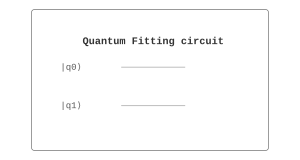
\includegraphics[width=0.6\textwidth]{../../images/quantum_fitting_circuit.svg}
\end{center}

\subsection{数学推导}

量子曲线拟合：
\begin{equation}
f(x) = \sum_k c_k \phi_k(x)
\end{equation}

\textbf{损失函数}：
\begin{equation}
L(c) = \sum_i (y_i - f(x_i))^2
\end{equation}

\subsection{几何解释}

量子曲线拟合在量子态空间中搜索最优参数。量子叠加允许同时探索多个参数组合。

\section{代码详解}

\begin{verbatim}
from quonic.ml import quantum_fitting

# quantum_fitting(x, y, degree)
# x: 自变量
# y: 因变量
# degree: 多项式阶数
result = quantum_fitting(x, y, degree=2)

# result.coefficients: 拟合系数
# result.residual: 残差
print(f'Coefficients: {result.coefficients}')
\end{verbatim}

\section{进阶用法}

\subsection{场景 1：不同阶数}

\begin{verbatim}
from quonic.ml import quantum_fitting

# 不同阶数
for d in [1, 2, 3]:
    result = quantum_fitting(x, y, degree=d)
    print(f'degree={d}: {result.coefficients}')
\end{verbatim}

\section{适用场景}

\subsection{数据拟合}

量子曲线拟合可以用于拟合实验数据。例如，拟合光谱数据、拟合时间序列数据等。量子叠加可以同时探索多个参数组合，加速拟合过程。

\subsection{函数逼近}

量子曲线拟合可以用于函数逼近。例如，逼近复杂函数、插值、外推等。量子曲线拟合可以利用量子核函数表示更复杂的函数。

\section{常见问题}

\subsection{量子曲线拟合和经典曲线拟合有什么区别？}

量子曲线拟合使用量子策略，可以利用量子叠加探索更大的参数空间。

\subsection{量子曲线拟合的精度如何？}

精度取决于多项式的阶数和数据的质量。

\section{学习路径}

\subsection{前置知识}
\begin{itemize}
  \item 曲线拟合
  \item 量子神经网络
  \item 量子测量
\end{itemize}

\subsection{继续学习}
\begin{itemize}
  \item 量子机器学习
  \item 量子回归
  \item 量子优化
\end{itemize}

\section{完整示例代码}

\subsection{示例 1：基本量子曲线拟合}

\begin{verbatim}
from quonic.ml import quantum_fitting

x = [0, 1, 2, 3]
y = [0, 1, 4, 9]
result = quantum_fitting(x, y, degree=2)
print(f'Coefficients: {result.coefficients}')
\end{verbatim}

\section{下载}

\begin{itemize}
  \item [quantum\_fitting.py](https://github.com/ChrisLee0721/QuoNic/blob/main/examples/quantum_fitting/quantum_fitting.py)
\end{itemize}

\end{document}
